\begin{SCn}
    \scnheader{Предложения к включению}
    \scnhaselement{Пример формализации на SCg №1}
    \scnaddlevel{1}
        \scntext{исходный текст}{Сож — река в Европе, протекает по территории России, Беларуси и частично по границе с Украиной. Левый приток Днепра. Длина реки — 648 км (из них 493 км по Беларуси), площадь её водосборного бассейна — 42 100 км\(^{2}\). Основные притоки: Вихра, Остёр, Проня, Беседь, Ипуть. Длина судоходного участка реки — 373 км. Ранее на Соже действовала шлюзованная система, разрушенная во время Великой Отечественной войны.На реке стоят следующие города: (вниз по течению): Кричев, Чериков, Славгород, Чечерск, Ветка, Гомель.}
        \scnrelfrom{SCg}{
            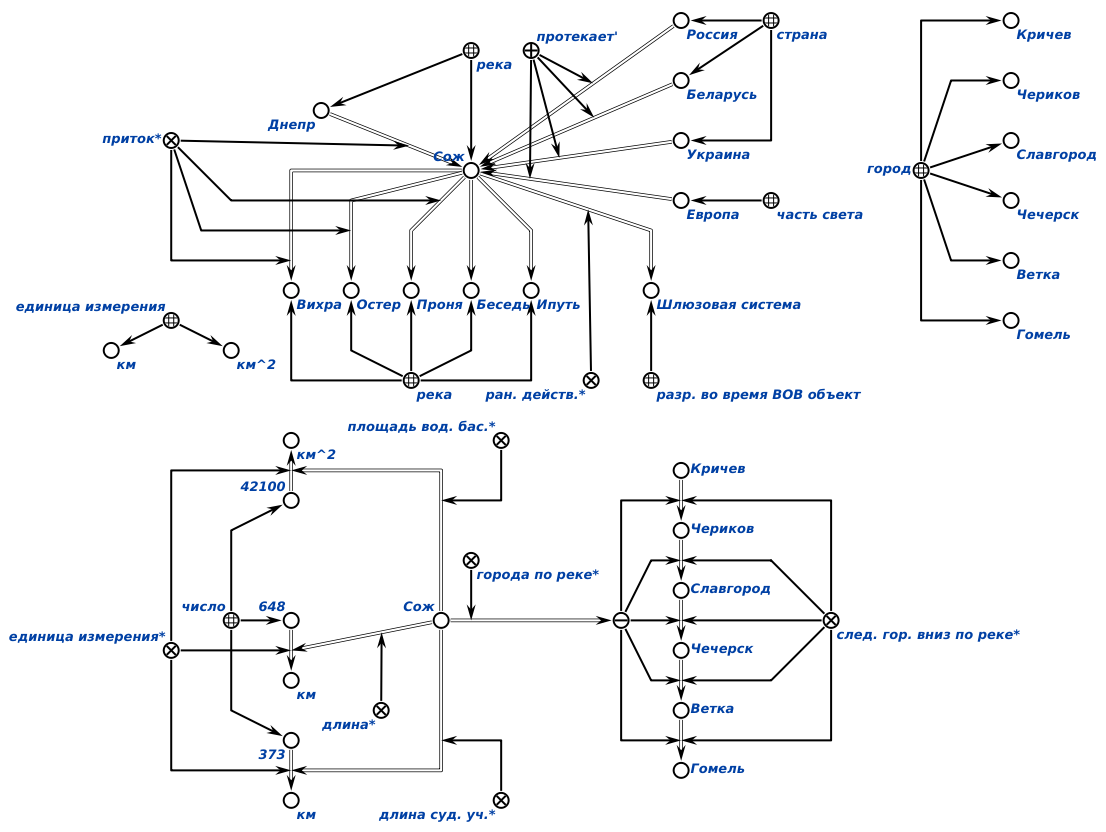
\includegraphics[scale=0.5]{images/work.png}
        }
    \scnaddlevel{-1}
    ~\\~\\~\\~\\
    \scnhaselement{Пример формализации на SCg №2}
    \scnaddlevel{1}
        \scntext{исходный текст}{ \(tg(3\alpha)=\frac{3tg\alpha-tg^{3}\alpha}{1-3tg^{2}\alpha}\) }
        \scnrelfrom{SCg}{
            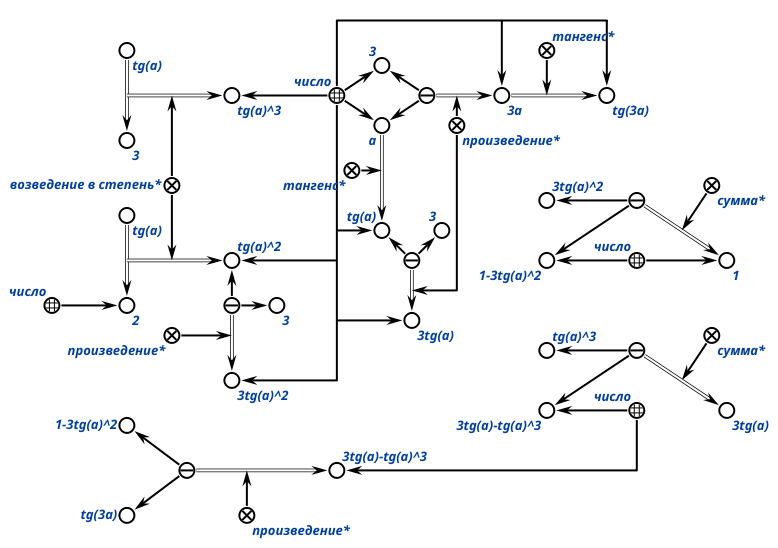
\includegraphics[scale=0.7]{images/work2.png}
        }
    \scnaddlevel{-1}
    \pagebreak
    \scnhaselement{Пример формализации на SCg №3}
    \scnaddlevel{1}
        \scntext{исходный текст}{ \(V = \frac{1}{3}{\pi}h(r^2_1+r_1r_2+r^2_2)\) }
        \scnrelfrom{SCg}{
            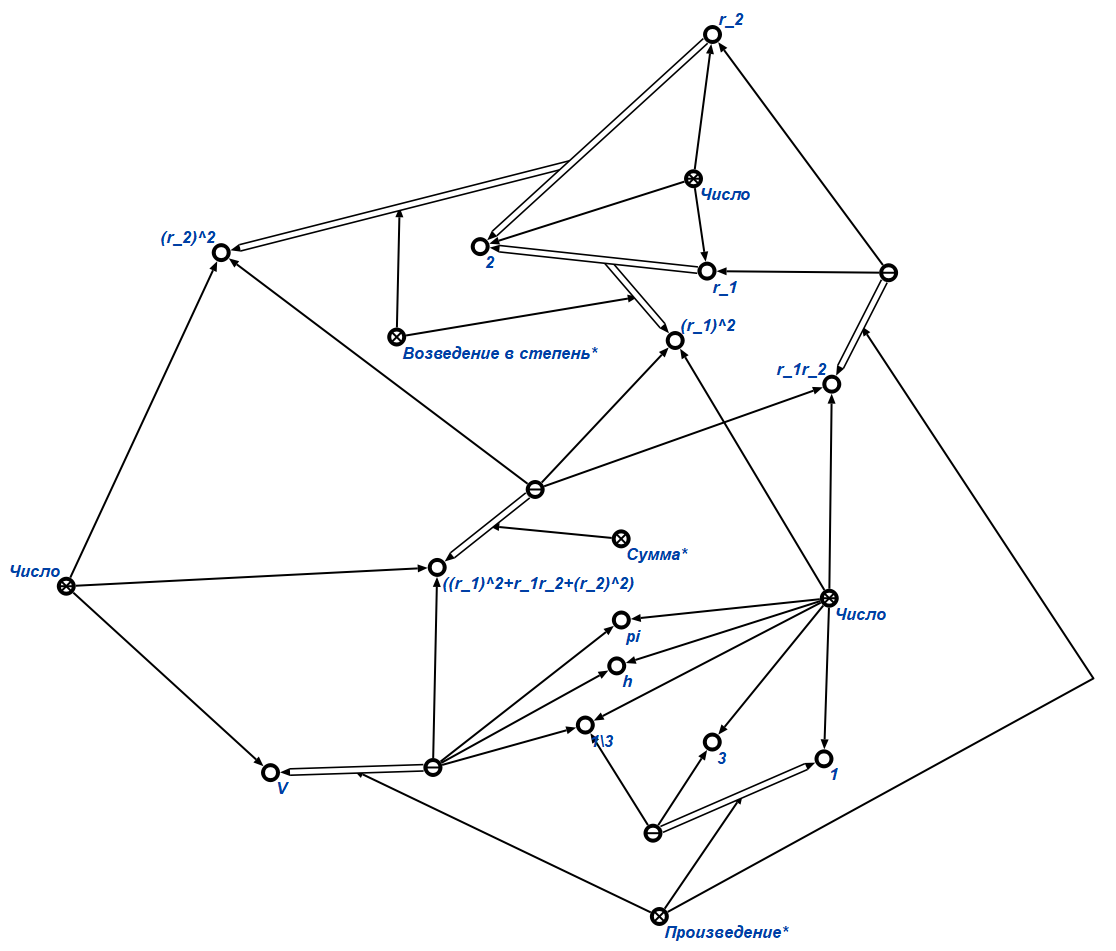
\includegraphics[scale=0.7]{images/ytsu.png}
        }
    \scnaddlevel{-1}
    \pagebreak
    \scnhaselement{Пример формализации на SCg №4}
    \scnaddlevel{1}
        \scntext{исходный текст}{Дан треугольник АВС. Периметр треугольника АВС равен 20 см. MN – средняя линия, параллельная стороне АС. MN лежит против угла B, градусная мера которого составляет половину градусной меры угла С. Медиана BK пересекает MN в точке О, АО = СО.}
        \scnrelfrom{SCg}{
            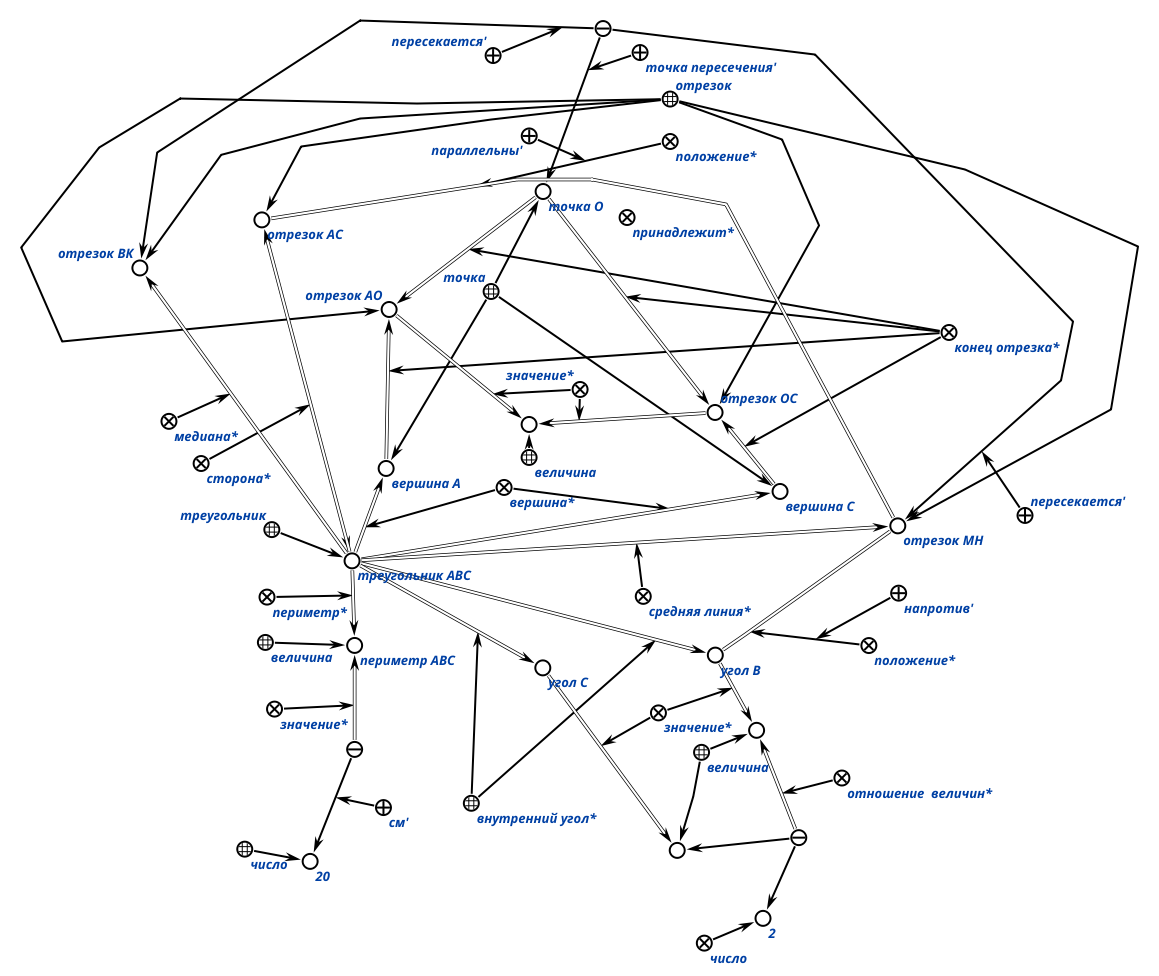
\includegraphics[scale=0.5]{images/sr.png}
        }
    \scnaddlevel{-1}
\end{SCn}